
% !TeX spellcheck = de_DE
\documentclass{article}

\usepackage[ngerman]{babel}
\usepackage{graphicx}
\usepackage{float}
\usepackage{booktabs}
\usepackage{lscape}
\usepackage{longtable}
\usepackage{geometry}
\usepackage{caption}
\usepackage{subcaption}

\graphicspath{ {./images/} }
\setlength\parindent{0pt}

\setlength\LTleft{0pt}
\setlength\LTright{0pt}

\makeatletter
\newcommand{\sectionauthor}[1]{
	{\parindent 0em \large \scshape Autor: #1 \par \nobreak \vspace*{1em}}
	\@afterheading
}
\newcommand{\specification}[3]{
	{\parindent 0.5em \hangindent 3em \hypertarget{spec:#1:#2}{\textbf{/#1#2/}} #3 \par \nobreak \vspace*{0.5em}}
}
\makeatother

\title{BiBi - Validierungsbericht}
\date{\today\\v1.0}
\author{
	Ivan Charviakou\\
	León Liehr\\
	Jonas Picker\\
	Sergei Pravdin
}

\begin{document}

%--Titel----------------------------------------------------------------------------------------------------------------------------------------------------------------------------------
\maketitle
\begin{figure}[H]
	\centering
	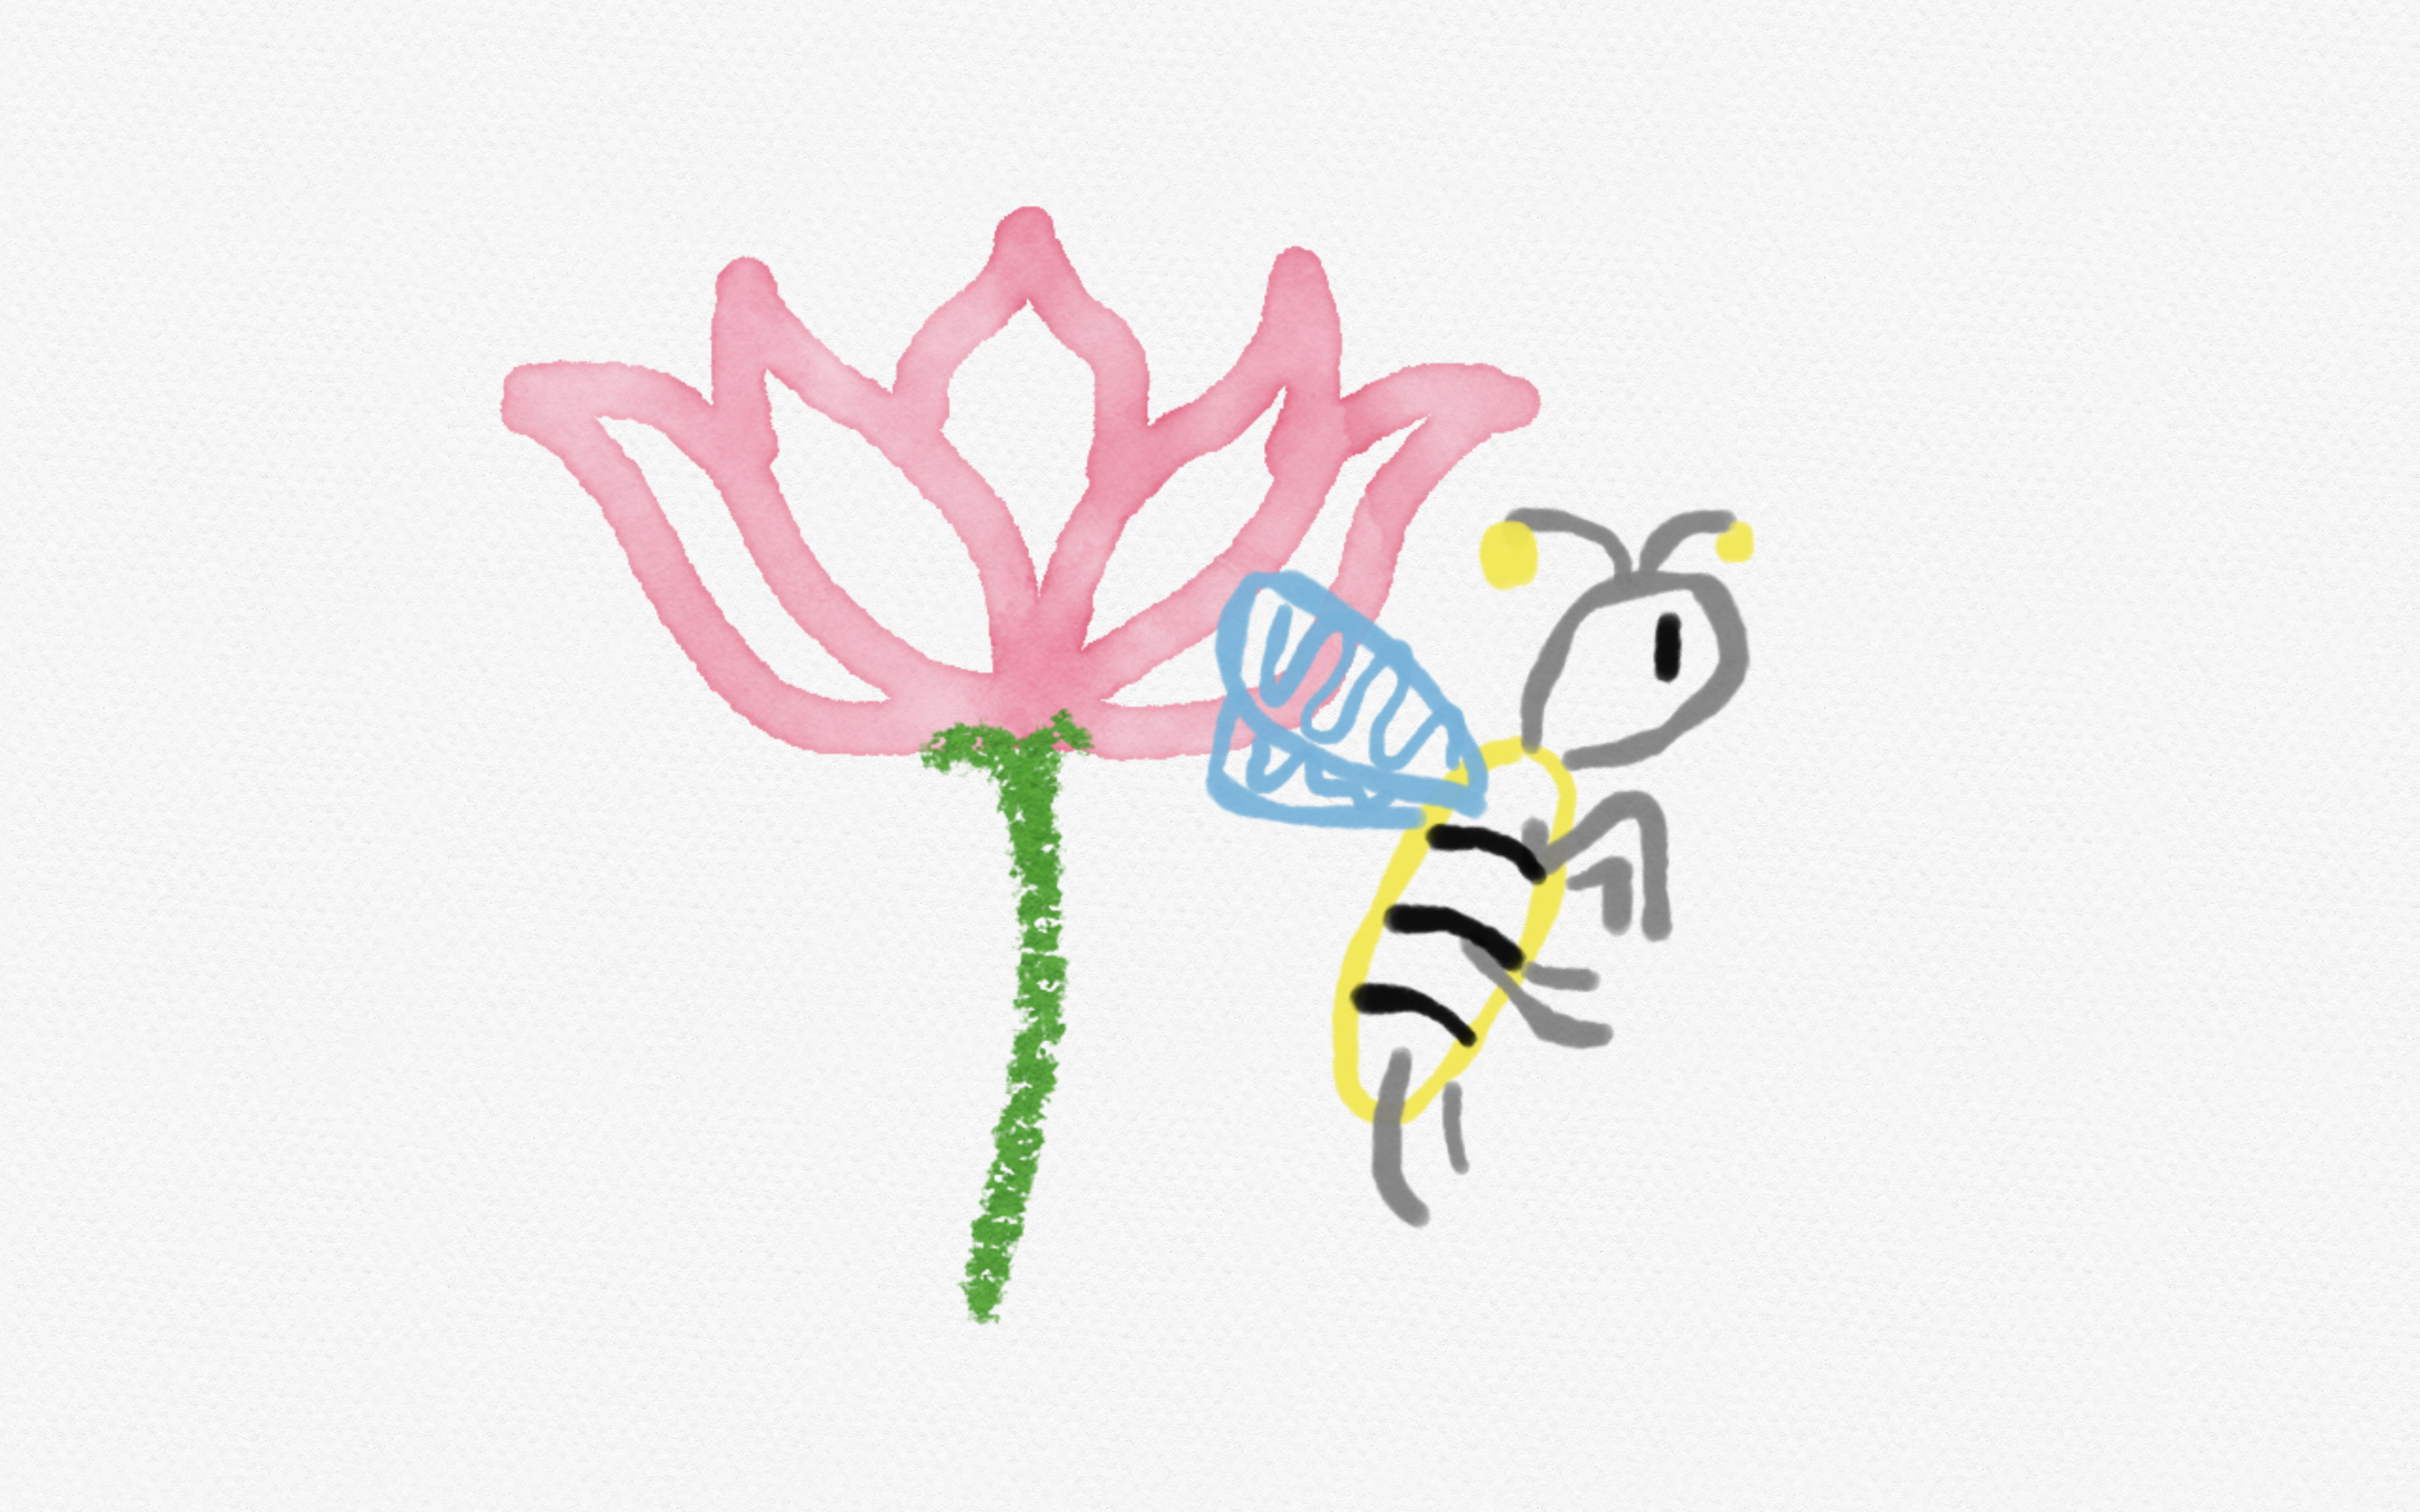
\includegraphics[width = 30em]{Logo}
\end{figure}
\newpage
\tableofcontents
\newpage

%--Einleitung--------------------------------------------------------------------------------------------------------------------------------------------------------------------------
\section{Einleitung}
\sectionauthor{Sergei Pravdin}



\newpage

%--Änderungen-----------------------------------------------------------------------------------------------------------------------------------------------------------------------
\section{Änderungen gegenüber dem Pflichtenheft}
\sectionauthor{Sergei Pravdin}



\newpage

%--Zusatztests-------------------------------------------------------------------------------------------------------------------------------------------------------------------------
\section{Zusätzliche Tests}
\sectionauthor{Jonas Picker}



\newpage

%--Testergebnisse--------------------------------------------------------------------------------------------------------------------------------------------------------------------
\section{Testergebnisse}
\sectionauthor{León Liehr}



\newpage

%--Überdeckungswerte--------------------------------------------------------------------------------------------------------------------------------------------------------------
\section{Überdeckungswerte}
\sectionauthor{Ivan Charviakou}



\newpage

%--Reference---------------------------------------------------------------------------------------------------------------------------------------------------------------------------
\section{Reference}
\sectionauthor{Wario}

\subsection{Nice looking table}
\begin{longtable}{@{}lllll@{}}
\toprule
\textbf{Header 1} & \textbf{Header 2} & \textbf{Header 3} & \textbf{Header 4} & \textbf{Header 5} \\* \midrule
\endfirsthead
%
\endhead
%
Text 1            & Text 2            & Text 3            & Text 4            & Text 5            \\
Text 1            & Text 2            & Text 3            & Text 4            & Text 5            \\* \bottomrule
\end{longtable}

\subsection{Nice looking landscape-table}
\begin{landscape}
\begin{longtable}{@{}lllll@{}}
\toprule
\textbf{Header 1} & \textbf{Header 2} & \textbf{Header 3} & \textbf{Header 4} & \textbf{Header 5} \\* \midrule
\endfirsthead
%
\endhead
%
Text 1            & Text 2            & Text 3            & Text 4            & Text 5            \\
Text 1            & Text 2            & Text 3            & Text 4            & Text 5            \\* \bottomrule
\end{longtable}
\end{landscape}

\newpage

\end{document}


